\documentclass[tikz, border=2mm]{standalone}
\usetikzlibrary{shapes.geometric} % for 3D shapes
\usetikzlibrary{3d} % for 3D coordinate transformation
\usetikzlibrary{perspective} % for perspective viewing

\begin{document}
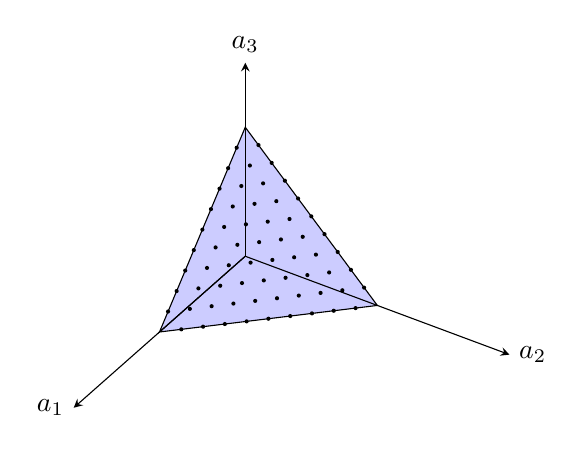
\begin{tikzpicture}[3d view={123}{35}] % Adjust these angles to change the viewing perspective
    \tikzstyle{point}=[circle, fill=black, minimum size=1.5pt, inner sep=0pt, outer sep=0pt]
    \draw[fill=blue!20] (0,0,0) -- (2,0,0) -- (0,2,0) -- (0,0,2) -- (2,0,0) -- cycle; % Tetrahedron
    % Add points to the faces

    \foreach \i in {0,0.1,...,1} {
        \foreach \j in {0,0.1,...,1} {
            \foreach \s in {0,0.1,...,1} {
            \pgfmathsetmacro\sumijk{\i+\j+\s}
            \ifdim\sumijk pt>0.98pt
                \ifdim\sumijk pt<1.01pt
                    \node[point] at (2*\i, 2*\j, 2*\s) {};
                \fi
            \fi
            }
        }
    }
    \begin{scope}
        \draw[-stealth] (0,0,0) -- (4,0,0) node[left] {$a_1$};
        \draw[-stealth] (0,0,0) -- (0,4,0) node[right] {$a_2$};
        \draw[-stealth] (0,0,0) -- (0,0,3) node[above] {$a_3$};
    \end{scope}
\end{tikzpicture}
\end{document}
